\section{Das elektrische Feld II}
\begin{flushleft}
\subsection{Das Konzept der Ladungsdichte}
\[
    \text{Raumladungsdichte: } \rho = \frac{dq}{dV}
\]\[
    \text{(Ober-)Flächenladungsdichte: } \sigma = \frac{dq}{dA}
\]\[
    \text{Linienladingsdichte: } \lambda = \frac{dq}{dl}
\]

Zur Berechnung der \textbf{Gesamtladung}: Integration über Volumen, Flächen resp. Kurven

\subsection{Berechnung von \texorpdfstring{$\Vec{E}$}{E}  mit dem Coulomb'schen Gesetz}

Ansatz: $dp = \rho dV$ wird als Punktladung betrachtet.
\[
\Rightarrow \text{$d\Vec{E} = \frac{1}{4\pi\epsilon_0}\frac{dq}{r^2}\hat{e}_r$}
\]
\begin{formulabox}
\[
    \Vec{E} = \int d\Vec{E} = \int_V \frac{1}{4\pi\epsilon_0}\frac{dq}{r^2}\hat{e}_r
\]
\end{formulabox}
\subsection{Das Gauss'sche Gesetz}

\textbf{Aussage:} Die Differenz aus der Anzahl der eine Oberfläche verlassenden und der in die Oberfläche eintrettenden Feldlinien ist proportional zu der von der Oberfläche eingeschlossenen \textbf{Gesamtladung}


\textbf{elektricher Fluss} für eine Ebenefäche mit beliebiger Orientierung:
\[
    \Phi_E = \Vec{E}\cdot\Vec{A} = \Vec{E}\cdot A\hat{n}
\]
Allgemein für den Gesamtfluss $\Phi_E$ gilt:
\begin{formulabox}
\[
    \Phi_E: \lim_{ \Delta A_i \to O} \sum_i \Vec{E}_i \Delta \Vec{A_i}  = \int_A \Vec{E}d\Vec{A} 
\]
\end{formulabox}
Mathematische Formulierung durch das Kreisintegral (geschlossene Oberfläche)
\begin{formulabox}
\[
    \Phi_E = \oint_A \Vec{E}d\Vec{A}
\]
\end{formulabox}
\textbf{Gauss'sches Gesetz}
\begin{formulabox}
\[
    \Phi_E = \oint_A \Vec{E}d\Vec{A} = \oint_A E_n dA = \frac{q_{innen}}{\epsilon_0} \hspace{1cm}  EA = \frac{Q}{\epsilon_0}
\]
\end{formulabox}


\subsection{Berechnung von \texorpdfstring{$\Vec{E}$}{E} mit dem Gauss'schen Gesetz}
\vspace{-1em}
\begin{multicols}{2}
\centering
   \textbf{$\Vec{E}$ für dünne Kugelschale:}
\begin{formulabox}
    \[
    \Vec{E}_r = \frac{1}{4\pi\epsilon_0}\frac{q}{r^2} \hspace{3mm}, (r > r_k)
    \]\[
    \Vec{E}_r = 0 \hspace{3mm}, (r < r_k)
    \]
\end{formulabox}

    \textbf{$\Vec{E}$ für homogen geladene Vollkugel:}
\begin{formulabox}
    \[
        \Vec{E}_r = \frac{1}{4\pi\epsilon_0}\frac{q}{r^2} \hspace{3mm}, (r > r_k)
    \]
    \[
        \Vec{E}_r = \frac{1}{4\pi\epsilon_0}\frac{q}{r_k^2}r \hspace{3mm}, (r < r_k)
    \]
\end{formulabox}
 
\end{multicols}

    \begin{center}
    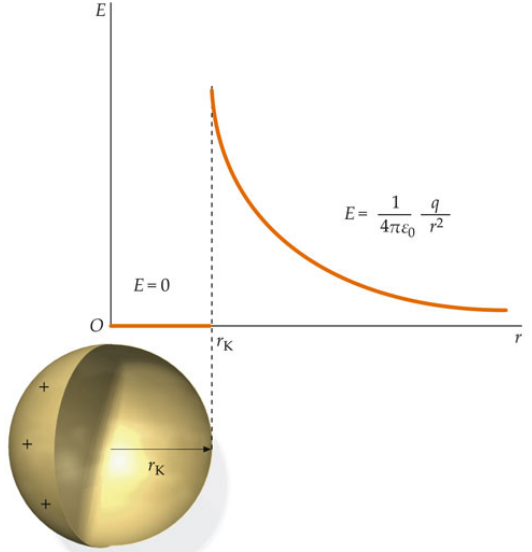
\includegraphics[width=0.34\linewidth]{Abbildungen Physik ZF/Gaussschens_Gesetz_dünne_Kugelschale.png}
    \hspace{5mm}
    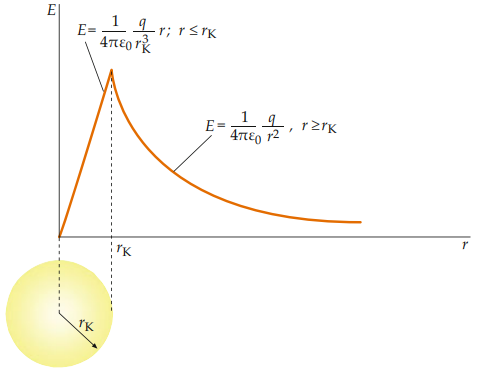
\includegraphics[width=0.45\linewidth]{Abbildungen Physik ZF/Gaussschens_Gesetz_Vollkugel.png}

    $\Vec{E}-Feld$ bei dünner Kugelschalen ist innerhalb immer = 0
    \end{center}

\subsection{Diskontinuität von \texorpdfstring{$E_n$}{En}}

\begin{center}
Unabhängig von der Form der Obergläche gilt:
\end{center}
\begin{formulabox}
    \[
    \Delta E_n = \frac{\sigma}{\epsilon_0}
    \]
\end{formulabox}
\begin{formulabox}
    \[
    \Delta E_n = E_{n,+} - E_{n,-} = \frac{\sigma}{2\epsilon_0} - \left(-\frac{\sigma}{2\epsilon_0}\right) = \frac{\sigma}{\epsilon_0}
    \]
\end{formulabox}
\subsection{Ladung \& Feld auf Leiteroberfläche}
Im elektrostatischen Gleichgewicht ist die Ladungsdichte und das $\Vec{E}-Feld$ im inneren eines Leiters überall = 0. \\
Das $\Vec{E}-Feld$ unmittelbar ausserhalb der Oberfläche hat keine tangentiale Komponente, nur Normalkomponente senkrecht zur Oberfläche mit: $E_n = \frac{\sigma}{\epsilon_0}$

\subsection{Das elektrische Potenzial}

\begin{formulabox}
    \[
    dE_{pot} = -\Vec{F} \cdot d\Vec{s}
    \]
\end{formulabox}
Für eine Punktladung $q_0$ gilt:
\begin{formulabox}
    \[
    dE_{pot} = dE_{el} = -q_0\Vec{E}\cdot d\Vec{s}
    \]
\end{formulabox}
Die Änderung der pot. Energie pro Ladungseinheit ist als Potenzialdifferenz definiert:
\begin{formulabox}
    \[
    d\phi = \frac{dE_{pot}}{q_0} = \frac{dE_{pot}}{q_0} = -\Vec{E} \cdot \Vec{s}
    \]
\end{formulabox}
Die Potenzialänderung bei Verschiebung von a nach b ist:
\begin{formulabox}
    \[
    \Delta\phi = \phi_b - \phi_a = \frac{\Delta E_{el}}{q_0} = - \int_b^a \Vec{E} \cdot d\Vec{s}
    \]
\end{formulabox}
Man wählt das elektr. Potenzial und die elektr. Energie so, dass sie im gleichen Bezugspunkt = 0 sind.
\begin{formulabox}
    \[
    E_{el} = q_0 \phi \hspace{7mm} [\phi] = \frac{J}{C} = V
    \]
\end{formulabox}
Die Potenzialdifferenz zwischen zwei Punkten wird auch (elektr.) Spannung genannt. \\
Es gilt: Das $\Vec{E}-Feld$ zeigt in die Richtung, in die das Potenzial $\phi$ am schnellsten abnimmt.

\subsection{Das Potenzial eines Punktladungsystems}
Für Punktladungen gilt: $\Vec{E} = \frac{1}{4\pi\epsilon_0} \frac{q}{r^2}\hat{e}_r$ \hspace{6mm} (B: Bezugspunkt ; P: beliebiger Punkt)
\[
    \phi_P - \phi_B = - \int_B^P \Vec{E}\cdot d\Vec{s} = -\int_B^P\frac{1}{4\pi\epsilon_0}\frac{q}{r^2}\hat{e}_r \cdot d\Vec{s} = -\int_B^P\frac{1}{4\pi\epsilon_0}\frac{q}{r^2}dr 
\]
\[
    \phi_P - \phi_B = \frac{1}{4\pi\epsilon_0}\frac{q}{r_P} - \frac{1}{4\pi\epsilon_0}\frac{q}{r_B}
\]
\\

Konvention: Bezugspunkt B im Unendlichen $\Rightarrow r_B \rightarrow \infty$
\begin{formulabox}
    \[
    \phi = \frac{1}{4\pi\epsilon_0}\frac{q}{r} \hspace{5mm} \text{Das Coulomb-Potenzial}
    \]
\end{formulabox}
\begin{formulabox}
    \[
    E_{el} = q_0\phi = \frac{1}{4\pi\epsilon_0}\frac{q_0 q}{r} \hspace{4mm} \text{elektr. Energie einer Punktladung}
    \]
\end{formulabox}
\begin{formulabox}
    \[
    \phi = \sum_i \frac{1}{4\pi\epsilon_0}\frac{q_i}{r_i} \hspace{3mm} \text{Potenzial eines Systems mit Superposition}
    \]
\end{formulabox}
\subsection{Berechnung des elektrischen Felds aus dem Potenzial}
Es gilt: $d\phi = -\Vec{E}\cdot\ d\Vec{s}$\\
\hspace{5mm} falls: $d\Vec{s} \perp \Vec{E}$ ist $d\phi$ = 0\\
\hspace{5mm} falls: $d\Vec{s} \parallel \Vec{E}$ ist $d\phi$ = maximal
\\[1ex]
Das $\Vec{E}-Feld$ ist gleich dem Negativen des Gradientes des Potenzials $\phi$
\begin{formulabox}
    \[
    \Vec{E} = -\nabla\phi = -\left(\frac{\partial\phi}{\partial x}\hat{e}_x + \frac{\partial\phi}{\partial y}\hat{e}_y + \frac{\partial\phi}{\partial z}\hat{e}_z\right)
    \]
\end{formulabox}

\subsection{Berechnung von \texorpdfstring{$\phi$}{phi} kontinuierlicher Ladungsverteilung}
Aus dem Superpositionsprinzip folgt: $\phi = \int \frac{1}{4\pi\epsilon_0}\frac{dq}{r}$\\
Annahme: Im Unendlichen Abstand von den Ladungen ist $\phi$ = 0.
\\[2ex]
\textbf{$\phi$ innerhalb \& ausserhalb einer homogenen geladenen Kugelschale:}
\begin{formulabox}
    \[
    \phi = -\int_{\infty}^{r_P} \frac{1}{4\pi\epsilon_0}\frac{q}{r^2}dr = \frac{1}{4\pi\epsilon_0}\frac{q}{r_P} \hspace{5mm} (r_P \geq r_K)
    \]
\end{formulabox}
$\Vec{E}$ innerhalb = 0; $\phi$ im inneren $\neq$ 0 !
\begin{formulabox}
    \[  
    \phi = -\int_{\infty}^{r_K} \frac{1}{4\pi\epsilon_0}\frac{q}{r^2}dr -\int_{r_K}^{r_P} \text{0} \ dr = \frac{1}{4\pi\epsilon_0}\frac{q}{r_K} \hspace{5mm} (r_P < r_K) 
    \]
\end{formulabox}

\subsection{Äquipotenzialflächen}
In einer Äquipotenzialfläche ist $\phi$ konstant. Feldlinien stehen immer senkrecht zu den Äquipotentialflächen.\\[1ex]
Jede Oberfläche eines Leiters ist eine Äquipotenzialfläche:
\[
    \phi = \frac{1}{4 \pi \epsilon_0}\frac{q}{r} \rightarrow q = 4 \pi r^2 \sigma \rightarrow \phi = \frac{1}{4 \pi \epsilon_0}\frac{4 \pi r^2 \sigma}{r} = \frac{r \sigma}{\epsilon_0} \rightarrow \sigma = \frac{\phi \epsilon_0}{r}
\]

\subsection{Die elektrische Energie}
Körper, die sich abstossen, besitzen eine höhere potenzielle Energie, wenn die näher beieinander sind. \\[1ex]
$\Rightarrow$ Arbeit wird verrichtet, um sie näher zu bringen \\[1ex]
Sich anziehende Körper haben die höchste potenzielle Energie, wenn sie weit voneinander entfernt sind.
\[
    \Rightarrow Arbeit: W = q \phi = q \frac{1}{4 \pi \epsilon_0}\frac{q}{r} = \frac{1}{4 \pi \epsilon_0}\frac{q_1 \cdot q_2}{r}
\]
\begin{formulabox}
    \[
     E_{el} = \frac{1}{2} \sum q_i \phi_i \hspace{3mm} \text{elektrische Energie eines Punktladungsystems}
    \]
\end{formulabox}

\end{flushleft}